

\chapter{Comets}

\begin{figure}[ht]
    %\vspace{-40pt}
    %\begin{adjustwidth}{-.9cm}{-0cm}
        \fbox{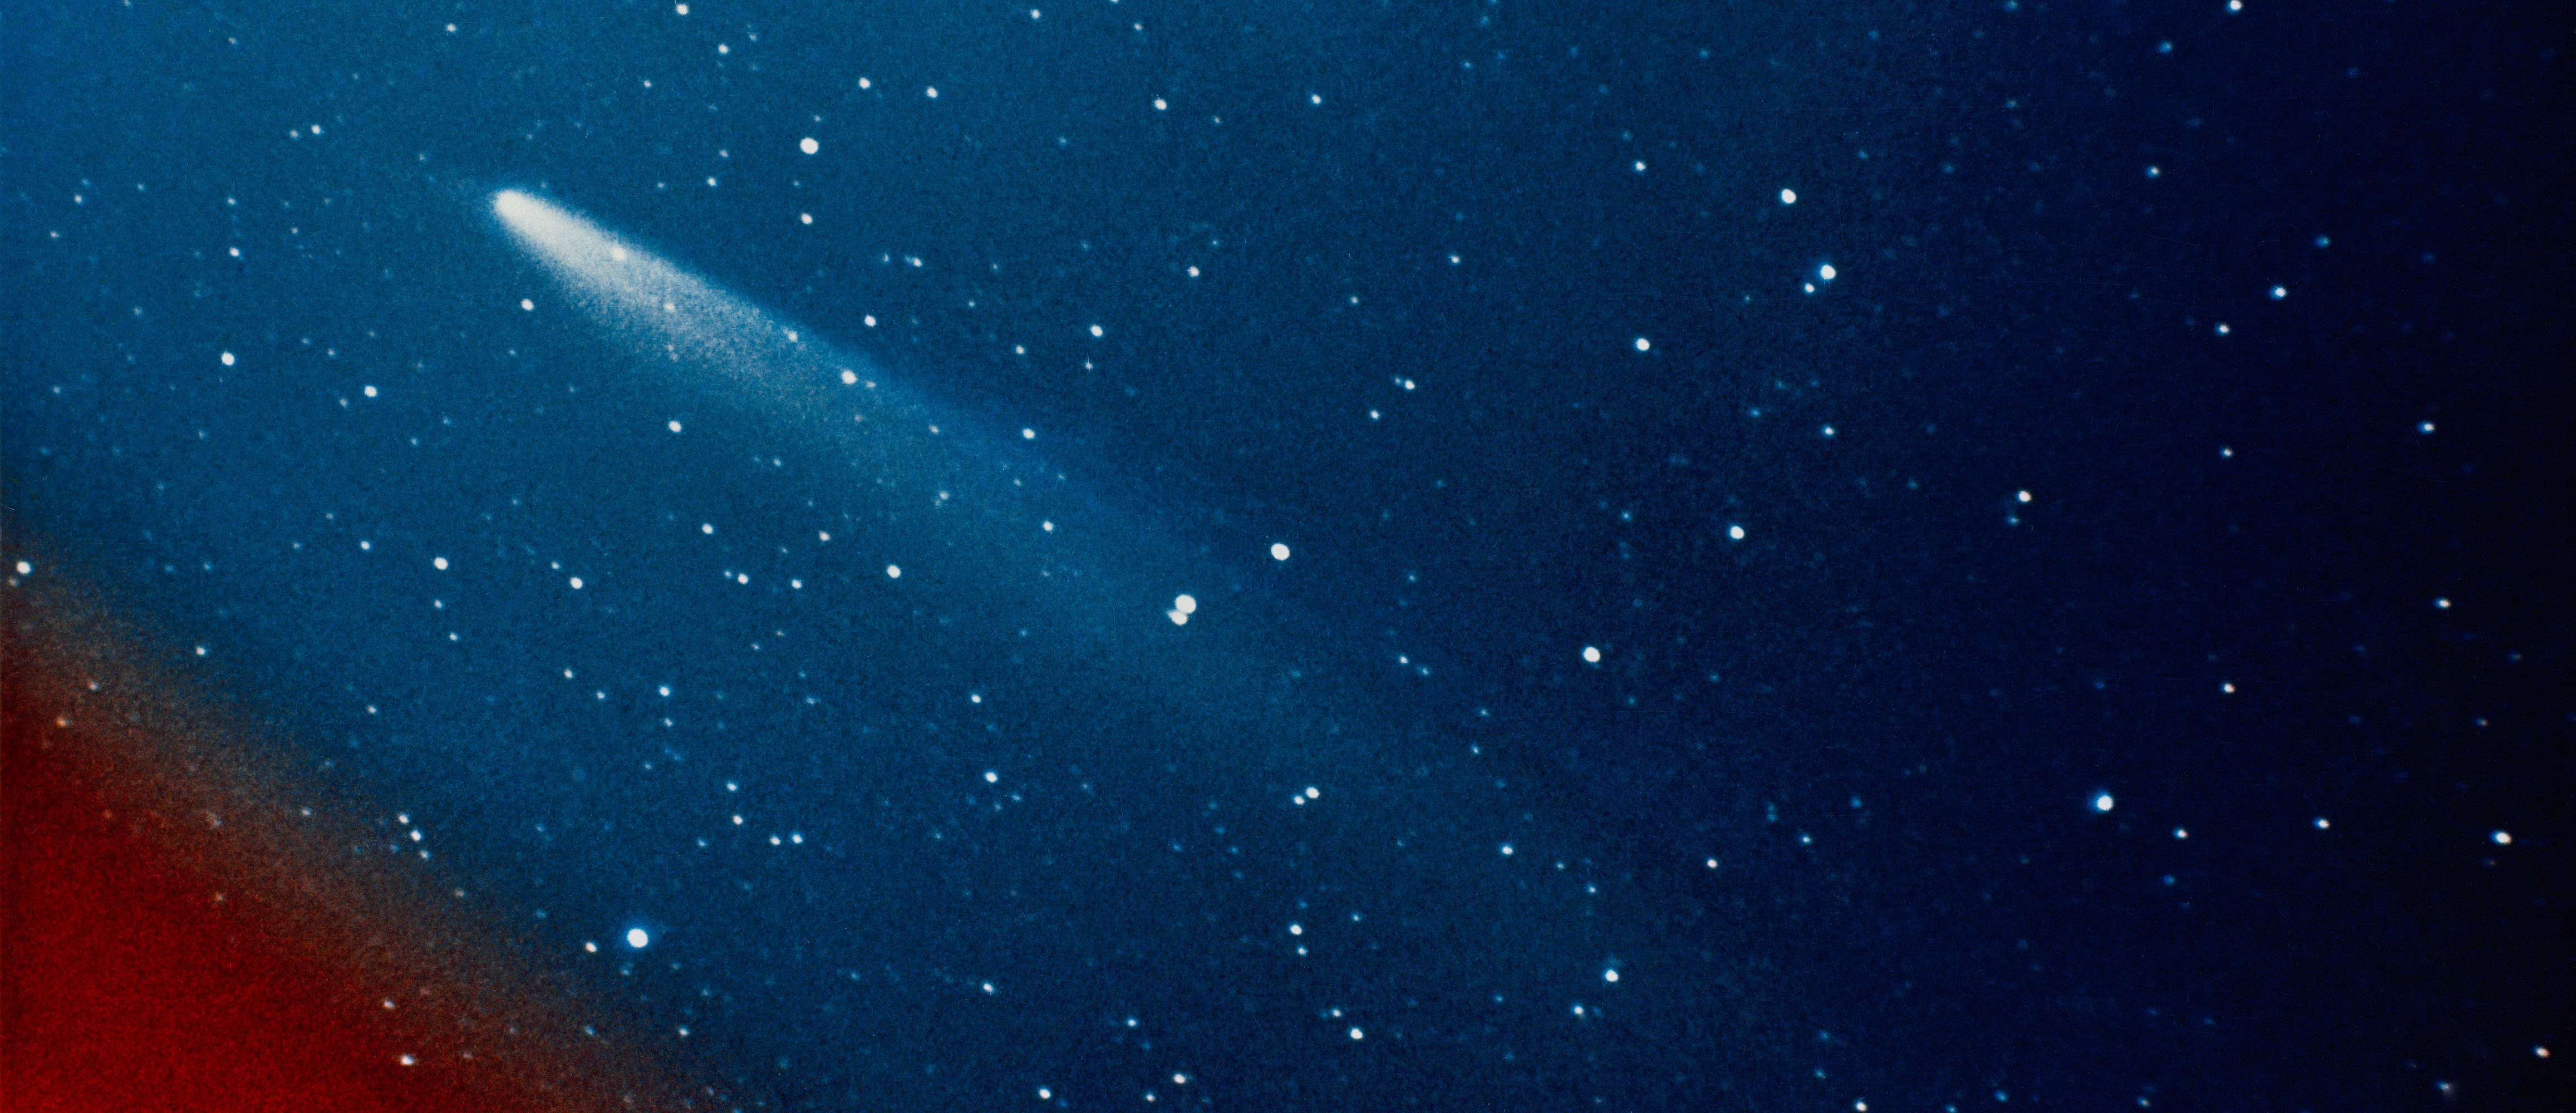
\includegraphics[width=\linewidth]{../../pictures/Comet_Kohoutek_(S74-17688)-2}}
        \captionsetup{width=\linewidth}
        \caption{\footnotesize Comet Kohoutek (C/1973 E1). Author: \href{https://pt.m.wikipedia.org/wiki/Ficheiro:Comet_Kohoutek_(S74-17688).jpg}{NASA}. Public domain.}
    %\end{adjustwidth}
\end{figure}

\lettrine[lines=4]{\goudy I}{t} seems highly probable that the period of rotation of all secondary planets is equal to that of their revolution round the main planet, and therefore that they always present to the latter the same side. Inequalities, occasioned by slight variations in the revolution, give rise to fluctuations of from 6 to 8, or to an apparent libration in longitude as well as in latitude. Thus, in the case of our moon, we sometimes observe more than half of its surface, with the eastern and northern edges being more visible at one time, and the western or southern at another. By means of this libration\footnote{Beer and Madler, op. cit., 185, s. 208, and 347, 8 332; and in their Phys. Kenntniss der himml. K\'{e}rper, s. 4 und 69, Tab. 1 (Physical History of the Heavenly Bodies).} we are enabled to see the annular mountain Malapert (which occasionally conceals the Moon's south pole), the arctic landscape round the crater of Gioja, and the large gray plain near Endymion, which exceeds in superficial extent the Mare Vaporum. Three sevenths of the Moon's surface are entirely concealed from our observation, and must always remain so, unless new and unexpected disturbing causes come into play. These cosmical relations involuntarily remind us of nearly similar conditions in the intellectual world, where, in the domain of deep research into the mysteries and the primeval creative forces of nature, there are regions similarly turned away from us, and apparently unattainable, of which only a narrow margin has revealed itself, for thousands of years, to the human mind, appearing, from time to time, either glimmering in true or delusive light. We have hitherto considered the primary planets, their satellites, and the concentric rings which belong to one, at least, of the outermost planets, as products of tangential force, and as closely connected together by mutual attraction. It therefore now only remains for us to speak of the unnumbered host of comets which constitute a portion of the cosmical bodies revolving in independent orbits round the Sun. If we assume an equable distribution of their orbits, and the limits of their perihelia, or greatest proximities to the Sun, and the possibility of their remaining invisible to the inhabitants of the Earth, and base our estimates on the rules of the calculus of probabilities, we shall obtain as the result an amount of myriads perfectly astonishing. Kepler, with his usual animation of expression, said that there were more comets in the regions of space than fishes in the depths of the ocean. As yet, however, there are scarcely one hundred and fifty whose paths have been calculated, if we may assume at six or seven hundred the number of comets whose appearance and passage through known constellations have been ascertained by more or less precise observations. While the so-called classical nations of the West, the Greeks and Romans, although they may occasionally have indicated the position in which a comet first appeared, never afford any information regarding its apparent path, the copious literature of the Chinese (who observed nature carefully, and recorded with accuracy what they saw) contains circumstantial notices of the constellations through which each comet was observed to pass. These notices go back to more than five hundred years before the Christian era, and many of them are still found to be of value in astronomical observations.\footnote{The first comets of whose orbits we have any knowledge, and which were calculated from Chinese observations, are those of 240 (under Gordian III.), 539 (under Justinian), 565, 568, 574, 837, 1337, and 1385. See John Russell Hind, in Schum., Astron. Nachr., 1843, No. 498. While the comet of 837 (which, according to Du S\'{e}jour, continued during twenty-four hours within a distance of 2,000,000 miles from the Earth) terrified Louis I. of France to that degree that he busied himself in building churches and Saati monastic establishments, in the hope of appeasing the evils threatened by its appearance, the Chinese astronomers made observations on the path of this cosmical body, whose tail extended over a space of 60, appearing sometimes single and sometimes multiple. The first comet that has been calculated solely from European observations was that of 1456, known as Halley's comet, from the belief long, but erroneously, entertained that the period when it was first observed by that astronomer was its first and only well-attested appearance. See Arago, in the Annuaire, 1836, p. 204, and Laugier, Comptes Rendus des S\'{e}ances de l'Acad., 1843, t. xvi., 1006.}

Although comets have a smaller mass than any other cosmical bodiesbeing, according to our present knowledge, probably not equal to s3;5th part of the Earths massyet theyoccupy the largest space, as their tails ia several instances extend over many millions of miles. The cone of luminous vapor which radiates from them has been found, in some eases in 1680 and 1811), to equal the length of the Earth's distance from the Sun, forming a line that intersects both theorbits of Venus and Mercury. It is even probable that thevapor of the tails of comets mingled with our atmosphere inthe years 1819 and 1823.

Comets exhibit such diversities of form, which appear rather to appertain to the individual than the class, that a description of one of these wandering light clouds, as they were already called by Xenophanes and Theon of Alexandria, contemporaries of Pappus, can only be applied with caution to another. The faintest telescopic comets are generally devoid of visible tails and resemble Herschel's nebulous stars. They appear like circular nebulae of faintly glimmering vapor, with the light concentrated toward the middle. This is the most simple type, but it cannot, however, be regarded as rudimentary since it might equally be the type of an older cosmical body, exhausted by exhalation. In the larger comets, we may distinguish both the so-called head or nucleus and the single or multiple tail, which is characteristically denominated by the Chinese astronomers as the brush (szz). The nucleus generally presents no definite outline, although, in a few rare cases, it appears like a star of the first or second magnitude and has even been seen in bright sunshine;\footnote{Arago, Annuaire, 1832, p. 209, 211. The phenomenon of the tail of a comet being visible in bright sunshine, which is recorded of the comet of 1402, occurred again in the case of the large comet of 1843, whose nucleus and tail were seen in North America on the 28th of February (according to the testimony of J. G. Clarke, of Portland, state of Maine), between 1 and 3 o'clock in the afternoon. The distance of the very dense nucleus from the sun's light admitted of being measured with much exactness. The nucleus and tail appeared like a very pure white cloud, a darker space intervening between the tail and the nucleus. (Amer. Journ. of Science, vol. xlv., No. 1, p. 229.)} as, for instance, in the large comets of 1402, 1532, 1577, 1744, and 1843. This latter circumstance indicates, in particular individuals, a denser mass, capable of reflecting light with greater intensity. Even in Herschel's large telescope, only two comets, that discovered in Sicily in 1807 and the splendid one of 1811, exhibited well-defined disks;\footnote{Phil. Trans. for 1808, Part ii., p. 155, and for 1812, Part i., p. 118.The diameters found by Herschel for the nuclei were 538 and 428 English miles. For the magnitudes of the comets of 1798 and 1805, seeArago, Annuaire, 1832, p. 203.

[The translator was at New Bedford, Massachusetts, U.S., on the 28th Februry, 1843, and distinctly saw the comet, between  and 2 in the afternoon. The sky at the time was intensely blue, and the sun shining with a dazzling brightness unknown in Europeas climates.] -- Tr.} the one at an angle of 1, and the other at 0.77, whence the true diameters are assumed to be 536 and 428 miles. The diameters of the less well-defined nuclei of the comets of 1798 and 1805 did not appear to exceed 24 or 28 miles.

In several comets that have been investigated with great care, especially in the above-named one of 1811, which continued visible for so long a period, the nucleus and its nebulous envelope were entirely separated from the tail by a darker space. The intensity of light in the nucleus of comets does not augment toward the center in any uniform degree, brightly shining zones being in many cases separated by concentric nebulous envelopes. The tails sometimes appear single, sometimes, although more rarely, double; and in the comets of 1807 and 1843, the branches were of different lengths; in one instance (1744), the tail had six branches, the whole forming an angle of 60. The tails have been sometimes straight, sometimes curved, either toward both sides or toward the side appearing to us as the exterior (as in 1811), or convex toward the direction in which the comet is moving (as in that of 1618); and sometimes the tail has even appeared like a flame in motion. The tails are always turned away from the sun, so that their line of prolongation passes through its center; a fact which, according to Edward Biot, was noticed by the Chinese astronomers as early as 837 but was first generally made known in Europe by Fracastoro and Peter Apian in the sixteenth century. These emanations may be regarded as conoidal envelopes of greater or less thickness, and, considered in this manner, they furnish a simple explanation of many of the remarkable optical phenomena already spoken of.

Comets are not only characteristically different in form, some being entirely without a visible tail, while others have a tail of immense length (as in the instance of the comet of 1618, whose tail measured 104), but we also see the same comets undergoing successive and rapidly changing processes of configuration. These variations of form have been most accurately and admirably described in the comet of 1744, by Hlensius, at St. Petersburg, and in Halley's comet, on its last reappearance in 1835, by Bessel, at Konigsberg. A more or less well-defined tuft of rays emanated from that part of the nucleus which was turned toward the Sun; and the rays being bent backward, formed a part of the tail. The nucleus of Halley's comet, with its emanations, presented the appearance of a burning rocket, the end of which was turned sideways by the force of the wind. The rays issuing from the head were seen by Arago and myself, at the Observatory at Paris, to assume very different forms on successive nights.\footnote{Arago, Des Changements physiques de la Comète de Halley du 1523 Oct., 1835. Annuaire, 1836, p. 218, 221. The ordinary direction of the emanations was noticed even in Nero's time. Come radios eos effugiunt. Seneca, Nat. Quest., vii., 20.} The great Konigsberg astronomer concluded from many measurements, and from theoretical considerations, that the cone of light issuing from the comet deviated considerably both to the right and the left of the true direction of the Sun, but that it always returned to that direction, and passed over to the opposite side, so that both the cone of light and the body of the comet from whence it emanated experienced a rotatory, or, rather, a vibratory motion in the plane of the orbit. He finds that the attractive force exercised by the Sun on heavy bodies is inadequate to explain such vibrations, and is of the opinion that they indicate a polar force, which turns one semidiameter of the comet toward the Sun, and strives to turn the opposite side away from that luminary. The magnetic polarity possessed by the Earth may present some analogy to this, and, should the Sun have an opposite polarity, an influence might be manifested, resulting in the precession of the equinoxes. This is not the place to enter more fully upon the grounds on which explanations of this subject have been based; but observations so remarkable,\footnote{Bessel, in Schumacher, Astr. Nachr., 1836, No. 300-302, s. 188, 192, 197, 200, 202, und 230. Also in Schumacher, Jahrb., 1837, s. 149, 168.William Herschel, in his observations on the beautiful comet of 1811,believed that he had discovered evidences of the rotation of the nucleusand tail (Pail. Trans. for 1812, Parti., p. 140). Dunlop, at Paramatla, thought the same with reference to the third comet of 1825.} and views of so exalted character, regarding the most wonderful class of the cosmical bodies belonging to our solar system, ought not to be entirely passed over in this sketch of a general picture of nature.

Although, as a rule, the tails of comets increase in magnitude and brilliance in the vicinity of the sun, and are directed away from that central body, yet the comet of 1823 offered the remarkable example of two tails, one of which was turned toward the sun, and the other away from it, forming with each other an angle of 160. Modifications of polarity and the unequal manner of its distribution, and of the direction in which it is conducted, may in this rare instance have occasioned a double, unchecked, continuous emanation of nebulous matter.\footnote{Bessel, in Astr. Nachr., 1836, No. 302, s. 231. Schum., Jahrb., 1837, s. 175. See, also, Lehmann, Ueber Cometenschweife (On the Tails of Comets), in Bode, Astron. Jahrb. far 1826, s. 168.}

Aristotle, in his Natural Philosophy, makes these emanations the means of bringing the phenomena of comets into a singular connection with the existence of the Milky Way. According to his views, the innumerable quantity of stars which compose this starry zone give out a self-luminous, incandescent matter. The nebulous belt which separates the different portions of the vault of heaven was therefore regarded by the Stagirite as a large comet, the substance of which was incessantly being renewed.\footnote{Aristot., Meteor., i., 8, 1114, und 1921 (ed. Ideler, t. i., p. 3234). Biese, Phil. des Aristoteles, bd. ii., s. 86. Since Aristotle exercised so great an influence throughout the whole of the Middle Ages, it is very much to be regretted that he was so averse to those grander views of the elder Pythagoreans, which inculcated ideas so nearly approximating to truth respecting the structure of the universe. He asserts that comets are transitory meteors belonging to our atmosphere in the very book in which he cites the opinion of the Pythagorean school, according to which these cosmical bodies are supposed to be planets having long periods of revolution. (Aristot., i., 6, 2.) This Pythagorean doctrine, which, according to the testimony of Apollonius Myndius, was still more ancient, having originated with the Chaldeans, passed over to the Romans, who in this instance, as was their usual practice, were merely the copiers of others. The Myndian philosopher describes the path of comets as directed toward the upper and remote regions of heaven. Hence Seneca says, in his Nat. Quest., vii., 17 "Cometes non est species falsa, sed proprium sidus sicut solis et lune altiora mundi secat et tunc demum apparet quum in imum cursum sui venit; and again (at vi'., 27), "Cometes aternos esse et sortis ejusdem, cujus cetera (sidera), etiamsi faciem illis non habent similem." Pliny (ii., 25) also refers to Apollonius Myndius, when he says, "Sunt qui et hec sidera perpetua esse credant suoque ambitu ire, sed non nisi relicta a sole cerni."}

The occultation of the fixed stars by the nucleus of a comet, or by its innermost vaporous envelopes, might throw some light on the physical character of these wonderful bodies; but we are unfortunately deficient in observations by which we may be assured\footnote{Olbers, in Astr. Nachr., 1828, s. 157, 184. Arago, De la Constitution physique des Comètes; Annuaire de 1832, p. 203, 208. The ancients were struck by the phenomenon that it was possible to see through comets as through a flame. The earliest evidence to be met with of stars having been seen through comets is that of Democritus (Aristot., Meteor., i., 6, 11), and the statement leads Aristotle to make the not unimportant remark, that he himself had observed the occultation of one of the stars of Gemini by Jupiter. Seneca only speaks devidedly of the transparency of the tail of comets. We may see, says he, stars through a comet as through a cloud (Nat. Quest., vii., 18); but we can only see through the rays of the tail, and not through the body of the comet itself zon in ea parte qua sidus ipsum est spissi et solidi ignis, sed qua rarus splendor occurrit et in crines dispergitur. Per intervalla ignium, non per ipsos, vides (vii., 26). The last remark is unnecessary, since, as Galileo observed in the Saggiatore (Lettera a Monsignor Cesarini, 1619), we can certainly see through a flame when it is not of too great a thickness.} that the occultation was perfectly central; for, as it has already been observed, the parts of the envelope contiguous to the nucleus are alternately composed of layers of dense or very attenuated vapor. On the other hand, the carefully conducted measurements of Bessel prove, beyond all doubt, that on the 29th of September, 1835, the light of a star of the tenth magnitude, which was then at a distance of 778 from the central point of the head of Halley's comet, passed through very dense nebulous matter, without experiencing any deflection during its passage.\footnote{Bessel, in the Astron. Nachr., 1836, No. 301, s. 204, 206. Struve, in Recueil des Mémoires de Acad. de St. Petersb., 1836, p. 140, 143, and Astr. Nachr., 1836, No. 303, s. 238, writes as follows: "At Dorpat the star was in conjunction only 22 from the brightest point of the comet. The star remained continually visible, and its light was not perceptibly diminished, while the nucleus of the comet seemed to be almost extinct before the radiance of the small star of the ninth or tenth magnitude."} If such an absence of refracting power must be ascribed to the nucleus of a comet, we can scarcely regard the matter composing comets as a gaseous fluid. The question here arises whether this absence of refracting power may not be owing to the extreme tenuity of the fluid; or does the comet consist of separated particles, constituting a cosmical stratum of clouds, which, like the clouds of our atmosphere, that exercise no influence on the zenith distance of the stars, does not affect the ray of light passing through it? In the passage of a comet over a star, a more or less considerable diminution of light has often been observed; but this has been justly ascribed to the brightness of the ground from which the star seems to stand forth during the passage of the comet.

The most important and decisive observations that we possess on the nature and the light of comets are due to Arago's polarization experiments. His polariscope instructs us regarding the physical constitution of the Sun and comets, indicating whether a ray that reaches us from a distance of many millions of miles transmits light directly or by reflection; and if the former, whether the source of light is a solid, a liquid, or a gaseous body. His apparatus was used at the Paris Observatory in examining the light of Capella and that of the great comet of 1819. The latter showed polarized, and therefore reflected light, while the fixed star, as was to be expected, appeared to be a self-luminous sun.\footnote{On the 3rd of July, 1819, Arago made the first attempt to analyze the light of comets by polarization, on the evening of the sudden appearance of the great comet. I was present at the Paris Observatory, and was fully convinced, as were also Matthieu and the late Bouvard, of the dissimilarity in the intensity of the light seen in the polariscope, when the instrument received cometary light. When it received light from Capella, which was near the comet, and at an equal altitude, the images were of equal intensity. On the reappearance of Halley's comet in 1835, the instrument was altered so as to give, according to Arago's chromatic polarization, two images of complementary colors (green and red). (Annales de Chimie, t. xill., p.108; Annuaire, 1832, p. 216.) We must conclude from these observations, says Arago, that the cometary light was not entirely composed of rays having the properties of direct light, there being light which was reflected specularly or polarized, that is, coming from the sun. It can not be stated with absolute certainty that comets shine only with borrowed light, for bodies, in becoming self-luminous, do not, on that account, lose the power of reflecting foreign light.} The existence of polarized cometary light announced itself not only by the inequality of the images, but was proved with greater certainty on the reappearance of Halley's comet, in the year 1835, by the more striking contrast of the complementary colors, deduced from the laws of chromatic polarization discovered by Arago in 1811. These beautiful experiments still leave it undecided whether, in addition to this reflected solar light, comets may not have light of their own. Even in the case of the planets, as, for instance, in Venus, an evolution of independent light seems very probable.

The variable intensity of light in comets cannot always be explained by the position of their orbits and their distance from the Sun. It would seem to indicate, in some individuals, the existence of an inherent process of condensation, and an increased or diminished capacity of reflecting borrowed light. In the comet of 1618, and in that which has a period of three years, it was observed first by Hevelius that the nucleus of the comet diminished at its perihelion and enlarged at its aphelion, a fact which, after remaining long unheeded, was again noticed by the talented astronomer Valz at Nimes. The regularity of the change of volume, according to the different degrees of distance from the Sun, appears very striking. The physical explanation of the phenomenon cannot, however, be sought in the condensed layers of cosmical vapor occurring in the vicinity of the Sun, since it is difficult to imagine the nebulous envelope of the nucleus of the comet to be vesicular and impervious to the ether.\footnote{Arago, in the Annuaire, 1832, p. 217-220. Sir John Herschel, Astron., 488.}

The dissimilar eccentricity of the orbits of comets has, in recent times (1819), in the most brilliant manner enriched our knowledge of the solar system. Encke has discovered the existence of a comet of so short a period of revolution that it remains entirely within the limits of our planetary system, attaining its aphelion between the orbits of the smaller planets and that of Jupiter. Its eccentricity must be assumed at 0.845, that of Juno (which has the greatest eccentricity of any of the planets) being 0.255. Encke's comet has several times, although with difficulty, been observed by the naked eye, as in Europe in 1819, and, according to Rümker, in New Holland in 1822. Its period of revolution is about 3.1 years; but, from a careful comparison of the epochs of its return to its perihelion, the remarkable fact has been discovered that these periods have diminished in the most regular manner between the years 1786 and 1838, the diminution amounting, in the course of 52 years, to about 1/4th days. The attempt to bring into unison the results of observation and calculation in the investigation of all the planetary disturbances, with the view of explaining this phenomenon, has led to the adoption of the very probable hypothesis that there exists dispersed in space a vaporous substance capable of acting as a resisting medium. This matter diminishes the tangential force, and with it the major axis of the comet's orbit. The value of the constant of the resistance appears to be somewhat different before and after the perihelion; and this may, perhaps, be ascribed to the altered form of the small nebulous star in the vicinity of the Sun, and to the action of the unequal density of the strata of cosmical ether.\footnote{Encke, in the Astronomische Nachrichten, 1843, No. 489, s. 130132.} These facts, and the investigations to which they have led, belong to the most interesting results of modern astronomy. Encke's comet has been the means of leading astronomers to a more exact investigation of Jupiter's mass (a most important point with reference to the calculation of perturbations); and, more recently, the source of this comet has obtained for us the first determination, although only an approximate one, of a smaller mass for Mercury. 

The discovery of Encke's comet, which had a period of only 31 years, was speedily followed, in 1826, by that of another, Biela's comet, whose period of revolution is 6.3 years, and which is likewise planetary, having its aphelion beyond the orbit of Jupiter, but within that of Saturn. It has a fainter light than Encke's comet, and, like the latter, its motion is direct, while Halley's comet moves in a course opposite to that pursued by the planets. Biela's comet presents the first certain example of the orbit of a comet intersecting that of the Earth. This position, with reference to our planet, may therefore be productive of danger, if we can associate an idea of danger with so extraordinary a natural phenomenon, whose history presents no parallel, and the results of which we are consequently unable correctly to estimate. Small masses endowed with enormous velocity may certainly exercise a considerable power; but Laplace has shown that the mass of the comet of 1770 is probably not equal to 1/25th of that of the Earth, estimating further with apparent correctness the mean mass of comets as much below 1/557th that of the Earth, or about 1/75th that of the Moon.\footnote{Laplace, Expos. du Syst. du Monde, p. 216, 237.} We must not confound the passage of Biela's comet through the Earth's orbit with its proximity to, or collision with, our globe. When this passage took place, on the 29th of October, 1832, it required a full month before the Earth would reach the point of intersection of the two orbits. These two comets of short periods of revolution also intersect each other, and it has been justly observed,\footnote{Littrow, Beschreibende Astron., 1835, s. 274. On the inner comet recently discovered by M. Faye, at the Observatory of Paris, and whose eccentricity is 0.551, its distance at its perihelion 1.690, and its distance at its aphelion 5.832, see Schumacher, Astron. Nachr., 1844, No. 495. Regarding the supposed identity of the comet of 1766 with the third comet of 1819, see Astr. Nachr., 1833, No. 239; and on the identity of the comet of 1743 and the fourth comet of 1819, see No. 237 of the last-mentioned work.} that amid the many perturbations experienced by such small bodies from the larger planets, there is a possibility, supposing a meeting of these comets to occur in October, that the inhabitants of the Earth may witness the extraordinary spectacle of an encounter between two cosmical bodies, and possibly of their reciprocal penetration and amalgamation, or of their destruction by means of exhausting emanations. Events of this nature, resulting either from deflection occasioned by disturbing masses or primevally intersecting orbits, must have been of frequent occurrence in the course of millions of years in the immeasurable regions of ethereal space; but they must be regarded as isolated occurrences, exercising no more general or alterative effects on cosmical relations than the breaking forth or extinction of a volcano within the limited sphere of our Earth.

A third interior comet, having likewise a short period of revolution, was discovered by Faye on the 22nd of November, 1843, at the Observatory at Paris. Its elliptic path, which approaches much more nearly to a circle than that of any other known comet, is included within the orbits of Mars and Saturn. This comet, therefore, which, according to Goldschmidt, passes beyond the orbit of Jupiter, is one of the few whose perihelia are beyond Mars. Its period of revolution is 728 years, and it is not improbable that the form of its present orbit may be owing to its great approximation to Jupiter at the close of the year 1839.

If we consider the comets in their enclosed elliptic orbits as members of our solar system, and with respect to the length of their major axes, the amount of their eccentricity, and their periods of revolution, we shall probably find that the three planetary comets of Encke, Biela, and Faye are most nearly approached in these respects, first, by the comet discovered in 1766 by Messier, and which is regarded by Clausen as identical with the third comet of 1819; and, next, by the fourth comet of the last-mentioned year, discovered by Blaupain, but considered by Clausen as identical with that of the year 1743, and whose orbit appears, like that of Lexell's comet, to have suffered great variations from the proximity and attraction of Jupiter. The two last-named comets would likewise seem to have a period of revolution not exceeding five or six years, and their aphelia are in the vicinity of Jupiter's orbit. Among the comets that have a period of revolution of from seventy to seventy-six years, the first in point of importance with respect to theoretical and physical astronomy is Halley's comet, whose last appearance, in 1835, was much less brilliant than was to be expected from preceding ones; next we would notice Olbers's comet, discovered on the 6th of March, 1815; and, lastly, the comet discovered by Pons in the year 1812, and whose elliptic orbit has been determined by Encke. The two latter comets were invisible to the naked eye. We now know with certainty of nine returns of Halley's large comet, it having recently been proved by Laugier's calculations,\footnote{Laugier, in the Comptes Rendus des S\'{e}ances de l'Academie, 1843, t. xvi., p. 1006.} that in the Chinese table of comets, first made known to us by Edward Biot, the comet of 1378 is identical with Halley's; its periods of revolution have varied in the interval between 1378 and 1835 from 7491 to 7758 years, the mean being 761. A host of other comets may be contrasted with the cosmical bodies of which we have spoken, requiring several thousand years to perform their orbits, which it is difficult to determine with any degree of certainty. The beautiful comet of 1811 requires, according to Argelander, a period of 3065 years for its revolution, and the colossal one of 1680 as much as 8800 years, according to Encke's calculation. These bodies respectively recede, therefore, 21 and 44 times further than Uranus from the Sun, that is to say, 33,600 and 70,400 millions of miles. At this enormous distance the attractive force of the Sun is still manifested; but while the velocity of the comet of 1680 at its perihelion is 212 miles in a second, that is, thirteen times greater than that of the Earth, it scarcely moves ten feet in the second when at its aphelion. This velocity is only three times greater than that of water in most sluggish European rivers, and equal only to half that which I have observed in the Cassiquiare, a branch of the Orinoco. It is highly probable that, among the innumerable host of uncalculated or undiscovered comets, there are many whose major axes greatly exceed that of the comet of 1680. In order to form some idea by numbers, I do not say of the sphere of attraction, but of the distance in space of a fixed star, or other sun, from the aphelion of the comet of 1680 (the furthest receding cosmical body with which we are acquainted in our solar system), it must be remembered that, according to the most recent determinations of parallaxes, the nearest fixed star is full 250 times further removed from our sun than the comet in its aphelion. The comet's distance is only 44 times that of Uranus, while  Centauri is 11,000, and 64Cygni 31,030 times that of Uranus, according to Bessels Jeterminations.

Having considered the greatest distances of comets from the central body, it now remains for us to notice instances of the greatest proximity hitherto measured. Lexell and Burckhardts comet of 1770, so celebrated on account of the disturbances it experienced from Jupiter, has approached the Earthwithin a smaller distance than any other comet. On the 28thof June, 1770, its distance from the Earth was only six timesthat of the Moon. The same comet passed twice, viz., in1769 and 1779, through the system of Jupiters four satelliteswithout producing the slightest notable change in the wellknown orbits of these bodies. The great comet of 1680 approached at its perihelion eight or nine times nearer to thesurface of the. Sun than Lexells comet did to that of ourEarth, being on the 17th of December a sixth part of theSuns diameter, or seven tenths of the distance of the Moonfrom that luminary. Perihelia occurring beyond the orbit ofMars can seldom be observed by the inhabitants of the Earth,owing to the faintness of the light of distant comets; andamong those already calculated, the comet of 1729 is the onlyone which has its perihelion between the orbits of Pallas andJupiter ; it was even observed beyond the latter.

Since scientific knowledge, although frequently blended with vague and superficial views, has been more extensively diffused through wider circles of social life, apprehensions of the possible evils threatened by comets have acquired more weight as their direction has become more definite. The certainty that there are within the known planetary orbits comets which revisit our regions of space at short intervals, that great disturbances have been produced by Jupiter and Saturn in their orbits, by which such as were apparently harmless have been converted into dangerous bodies, the intersection of the Earth's orbit by Biela's comet, the cosmical vapor, which, acting as a resisting and impeding medium, tends to contract all orbits, the individual difference of comets, which would seem to indicate considerable decreasing gradations in the quantity of the mass of the nucleus, are all considerations more than equivalent, both as to number and variety, to the vague fears entertained in early ages of the general conflagration of the world by flaming swords and stars with fiery streaming hair. As the consolatory considerations which may be derived from the calculus of probabilities address themselves to reason and to meditative understanding only, and not to the imagination or to a desponding condition of mind, modern science has been accused, and not entirely without reason, of not attempting to allay apprehensions which it has been the very means of exciting. It is an inherent attribute of the human mind to experience fear, and not hope or joy, at the aspect of that which is unexpected and extraordinary.\footnote{Fries, Vorlesungen uber die Sternkunde, 1833, s. 262267 (Lectureson the Science of Astronomy). An infelicitously chosen instance of thegood omen of a comet may be found in Seneca, Nat. Quest., vii., 17 and21. The philosopher thus writes of the comet  Quem nos Neronisprincipatu letissimo vidimus et qui cometis detraxit infamiam.} The strange form of a large comet, its faint nebulous light, and its sudden appearance in the vault of heaven, have in all regions been almost invariably regarded by the people at large as some new and formidable agent inimical to the existing state of things. The sudden occurrence and short duration of the phenomenon lead to the belief of some equally rapid reflection of its agency in terrestrial matters, whose varied nature renders it easy to find events that may be regarded as the fulfillment of the evil foretold by the appearance of these mysterious cosmical bodies. In our own day, however, the public mind has taken another and more cheerful, although singular, turn with regard to comets; and in the German vineyards in the beautiful valleys of the Rhine and Moselle, a belief has arisen, ascribing to these once ill-omened bodies a beneficial influence on the ripening of the vine. The evidence yielded by experience, of which there is no lack in these days when comets may so frequently be observed, has not been able to shake the common belief in the meteorological myth of the existence of wandering stars capable of radiating heat.
